\cleardoublepage

\appendix
\addtocontents{lof}{\protect\setcounter{tocdepth}{0}}

\chapter{Statement of the Works Council}
\label{statement_br}
\begin{figure}[!h]
    \centering
    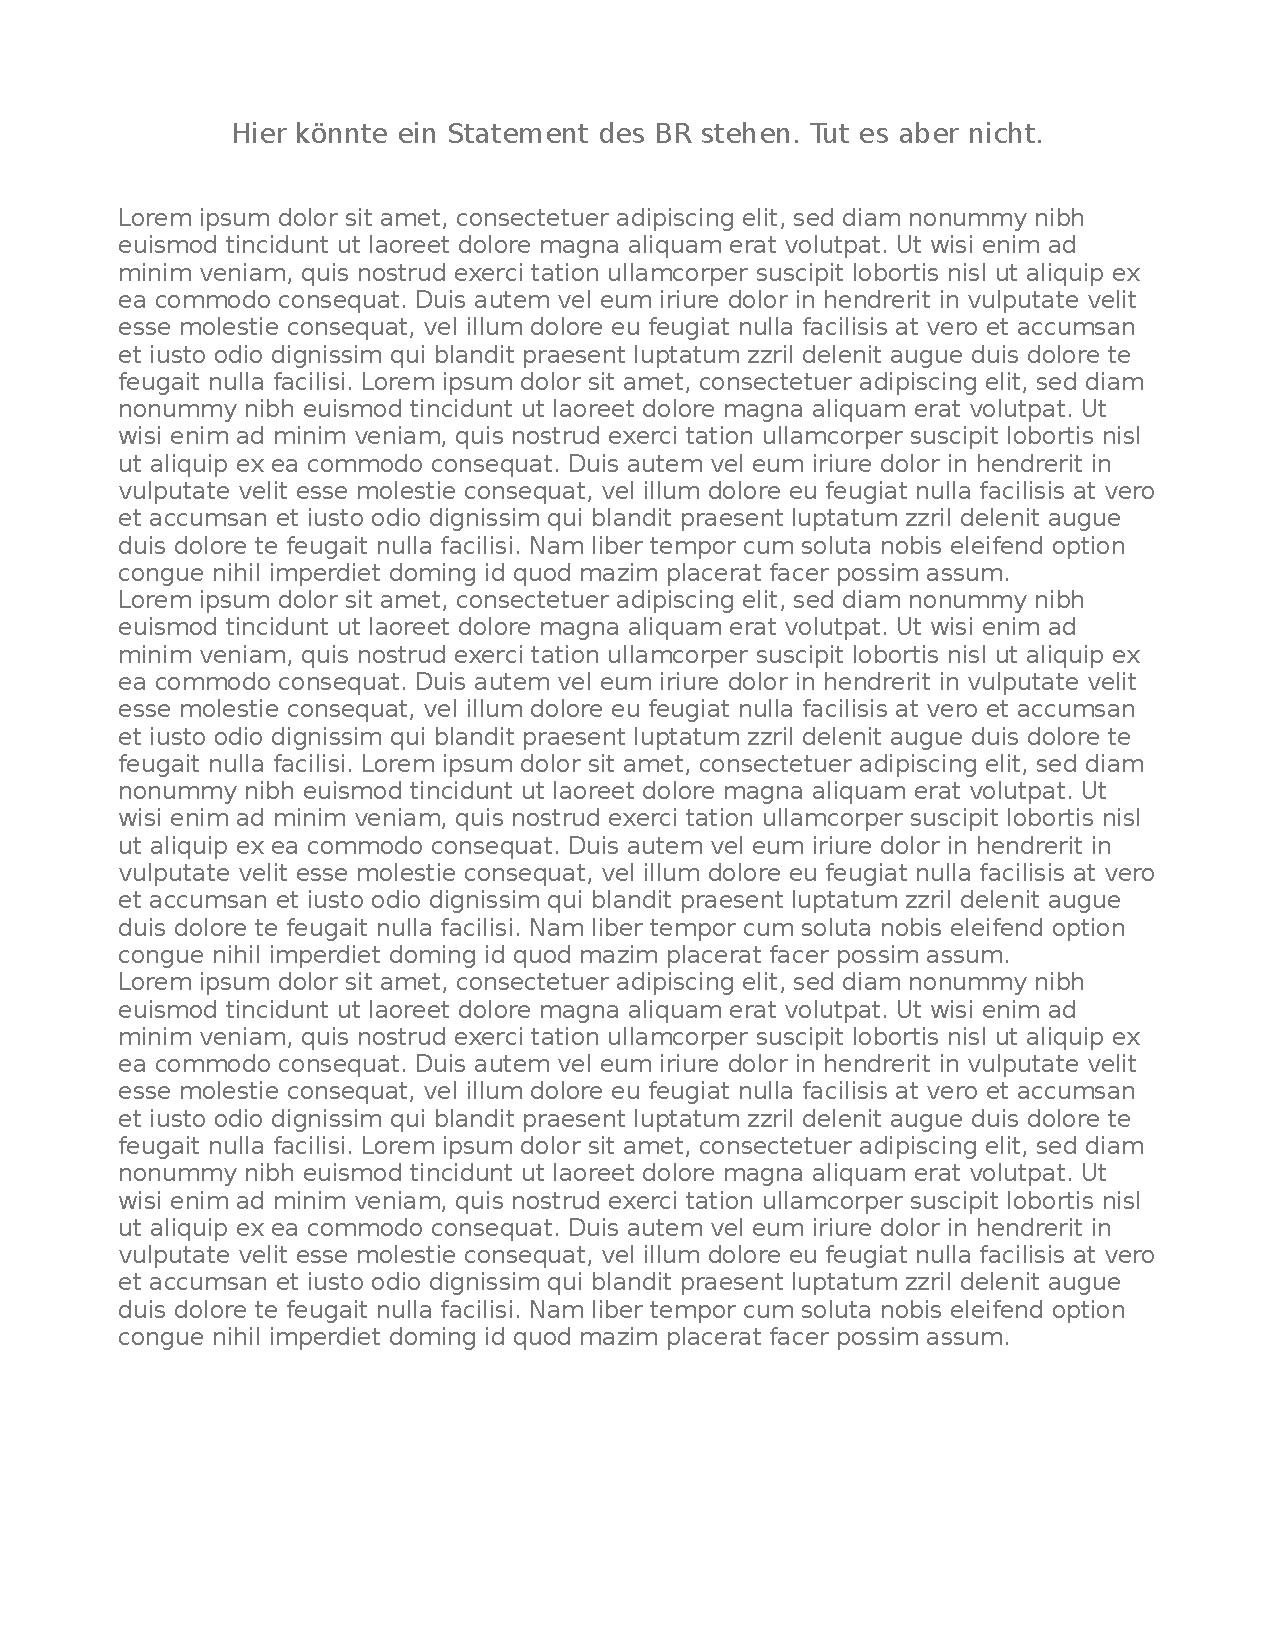
\includegraphics[width=0.9\textwidth,page=1]{images/statement_br.pdf}
    \caption[Statement of the Works Council]{Statement of the Works Council regarding mutual ratings.}
\end{figure}

\chapter{Interviews}

\section{Consent Form}
\label{consentform}
\begin{figure}[!h]
    \centering
    
\includegraphics[width=0.9\textwidth,page=1]{images/Interview_Consent.pdf}
    \caption[Interview Consent Form]{Interview Consent Form (Page 1)}
\end{figure}
\begin{figure}[!h]
    \centering
    
\includegraphics[width=0.9\textwidth,page=2]{images/Interview_Consent.pdf}
    \caption[]{Interview Consent Form (Page 2)}
\end{figure}

\newpage

\section{Transcripts (DE)}
\label{transcripts}
The interviews described in \ref{interviewquestions} have been recorded and transcripted. The transcripts can be found in this section.

\subsection{Mr. Gruber}
\begin{itemize}
\item[] \textit{Was wünscht du dir vom SkillWill Tool?}
\item[] Einen guten Überblick über die Erfahrungen der Mitarbeiter, ihre Wünsche in Bezug auf gewisse Skills, auch mal zu sehen, ob sie da Lust darauf haben, oder eben auch nicht. Und daraus dann ableiten können, wohin sich die Mitarbeiter entwicklen (sollen).

\item[] \textit{Dann haben wir gleich eine Anschlussfrage: Glaubst du bei den Wills soll mit Erfasst werden wie langfristig die sind? Also ob ich jetzt nur kurz Lust habe auf Java oder auf ewig?}
\item[] Ich denke mal nicht, dass wir eine Art Historie in dem Tool brauchen, sondern, dass das Tool ausreichend ist, wenn es den aktuellen Status protokolliert. Wenn sich Änderungen ergeben wird das im Tool festgehalten, aber ich brauche nicht die vorhergehenden Werte.

\item[] \textit{Aber auch keinen Blick in die Zukunft?}
\item[] Den leite ich dann tatsächlich mit dem Mitarbeiter zusammen davon ab.

\item[] \textit{Skills und Wills werden auf einer numerischen Skala angegeben, wie groß sollte diese sein?}
\item[] Von null bis fünf würde meiner Meinung nach ausreichen, man könnte das auch von minus zwei bis plus zwei über null aufziehen, weil der Wille ja auch negativ aussschlagend ist, da hättest du dann mit dem negativen Bereich eine Kennzeichnung, dass du da gar keine Lust drauf hast. Und das gleiche nochmal in positive ausschlagend. Null dann halt als neutrales Element.

\item[] \textit{Sollte die Gesamtberufserfahrung mit erfasst werden?}
\item[] Die Gesamtberufserfahrung, nein. Besondere Merkmale hingegen ja. Zum Beispiel wenn der Mitarbeiter eine Zertifizierung für eine spezielle Software hat, Beispiel AEM, wenn da eine Schulung mit gemacht wurde, das sind Informationen, die wir durchaus gebrauchen können.  Die langjährige Einschätzung, dafür sind die Vorgesetzten da, das muss nicht im Tool erfasst werden.

\item[] \textit{Zertifikate, wenn wir schon dabei sind: Als Skill erfassen, oder separat?}
\item[] Guter Punkt. Das wüsste ich so auf anhieb ehrlich gesagt nicht.

\item[] \textit{Sollte das Tool automatisch Teams erstellen können? Nach dem Motto “ich wünsche eine Team von vier Mann, die AEM, Java und was weiß ich” können und das Tool generiert dieses Team.}
\item[] Würde ich nicht als Bestandteil dieses Tools sehen, weil wir für das konkrete Erfassen der Projekte ein anderes Tool verwenden. Allerdings soll dieses Tool einen Impuls geben, wer wohin gehen könnte.
\item[] \textit{Sollten Mitarbeiter einander bewerten können?}
\item[] Nein.
\end{itemize}

\newpage

\subsection{Mr. Warnholz}
\begin{itemize}
\item[] \textit{Was wünscht du dir vom SkillWill Tool?}
\item[] Erstmal würde ich davon erwarten, dass mir das in meiner Arbeit als Account Manager die Arbeit erleichtert, um passende Mitarbeiter für meine Projekte zu finden.

\item[] \textit{Die Skill- Und Willlevel werden auf einer numerischen Skala von 0 bis n angegeben. Wie groß sollte n sein, damit es sinnvoll ist? Also wie groß soll die Skala sein?}
\item[] Ich würd sagen auf jeden Fall ungerade, ich würd sagen von eins bis fünf würde ausreichen.

\item[] \textit{Sollte die Gesamtberufserfahrung des Mitarbeiters in der suche mit einbezogen werden?}
\item[] Also indem man aktiv danach suche, oder als Ausgabe dann unter Namen usw.?

\item[] \textit{Das würde mit beim Namen angezeigt und je “senioriger” der Mitarbeiter, desto weiter oben in der Suche.}
\item[] Also gibts da schon eine Vorfilterung zu?

\item[] \textit{Genau das ist ja die Frage.}
\item[] Also würde es dann geben. Würde ich, glaub ich, hilfreich finden, ja.

\item[] \textit{Die Will Levels: Glaubst du da soll erfasst werden, ob das ein langfristiger Will ist, oder ein kurzfristiger?}
\item[] Auf jeden Fall glaube ich sollte irgendwo durch eine spätere, oder durch eine regelmäßige Abfrage oder Anpassung dieser Wills irgendwie eine synchronisation erfolgen. Weil, das kann ja sein, dass du mal vor dreizehn Monaten angegeben hast, dass du mal AEM besser entwickeln wollen würdest, nach neun Monaten bist du dann quasi auf dem “Expert Level”, aber da steht dann immernoch drin, und das willst du dann ja gar nicht mehr so dringend entwickeln oder dich weiterbilden, weil du das ja so gut kannst, aber in dem Tool steht dann immernoch drin, dass du dich da weiterentwickeln wollen würdest, das macht ja nicht so viel Sinn.

\textit{Die Idee war, dass das im Rahmen der Halbjahresgespräche gemacht wird.}
\item[] Würde wahrscheinlich für die erste Zeit erstmal ausreichen.

\item[] \textit{Fändest du es sinnvoll, wenn sich Mitarbeiter untereinander bewerten?}
\item[] Schwierig. Glaube nicht, als erster Impuls. Weil, da würden wahrscheinlich zu viele persönliche Befindlichkeiten mit Einfließen, also “mag ich den?”, “hatte ich mit dem schonmal eine weitergehende Beziehung als die professionelle bei der Arbeit?”, das kann alles da mit reinspielen. Also ich glaube da ist das schwierig dann irgendwo abzugrenzen, was professionell ist, oder was wirklich arbeitstechnisch relevant ist, und eben was einfach nur auf Sympathie oder Nicht-Symptathie beruht.

\item[] \textit{Und last but not least: Fändest du es sinnvoll, wenn das Tool automatisch Teams zusammen stellt? Nach dem Motto: “Ich möchte ein Team von vier Leuten, die zusammen Java und AEM und PHP können?”}
\item[] Why not? Könnte ich mir als sinnvoll vorstellen. Hätte ich unendlich Ressourcen, also unendlich Mitarbeiter, zur Verfügung, dann wäre es sehr wahrscheinlich, dass eine sinnvolle Zusammenstellung da rauskommt als Ergebnis. Bei der Ressourcensituation wie sie jetzt aber aktuell ist und sehr wahrscheinlich auch in Zukunft noch zugespitzter sein wird, wird das definitiv nie als Ergebnis rauskommen. Kann ich mir vorstellen. Oder bedenkt das Tool auch Verfügbarkeiten?

\item[] \textit{Nein.}
\item[] Gut, dann kannst du was ich vorher gesagt habe quasi streichen. Aber das ist dann das Ding, es würde dir wahrscheinlich nach den Anforderungen, die ich eingebe, ein sinnvolles Ergebnis geben, ob die dann aber verfügbar sind, ist eine ganz andere Frage. Und das wird wahrscheinlich ein bischen Schwierig sein.
\end{itemize}

\newpage

\subsection{Ms. Spranger}
\begin{itemize}
\item[] \textit{Was wünscht du dir vom SKillWill Tool?}
\item[] Ich wünsche mir, dass es einfach bedienbar ist, dass es viel genutzt wird, dass es einen Mehrwert bietet und die Teamplanung vereinfacht, dass es die Mitarbeiterentwicklung vereinfacht, also die Bedarfe und Wünsche besser aufzeigt und dass es uns eine bessere Übersicht verschafft.

\item[] \textit{Skill- und Willlevel werden auf einer Skala angegeben, wie groß sollte diese Skala sein?}
\item[] Ich würde sagen, vier unterschiedliche Werte reichen, denn es soll ja kein Mitarbeiterbewertungstool werden wo wir auf fünfzehn unterschiedlichen Skalenschritten angeben wie gut jemand ist, damit wir Leute vergleichen können, sondern wir wollen eine ganz ungefähre Tendenz bekommen, und genauer kriegt man es sowieso nicht hin.

\item[] \textit{Sollte die Gesamtberufserfahung mit erfasst werden? Und wenn ja, sollte das in der Suche berücksichtigt werden?}
\item[] Kann sicher nicht schaden, wäre die Frage, ob das zu personenbezogene Daten sind. Ob jemand Junior, Intermediate oder Senior ist, das sollte auf jeden Fall mit rein, die Anzahl an Berufsjahren, das weiß ich nicht.

\item[] \textit{Sollte das in der Suche mit berücksichtigt werden?}
\item[] Wenn ich nach einem bestimmten Skill suche, dann hab ich ja die Erfahrung über das Skill Level.

\item[] \textit{Aber wenn wir jetzt die generelle Berufserfahrung betrachten und nicht auf den einzelnen Skill?}
\item[] Ne, nicht immer ist mehr Jahre auch mehr Erfahrung. Deswegen nein. Da reicht es, wenn der Titel mit angezeigt wird, aber in der Suche macht das keinen Sinn.

\item[] \textit{Soll bei den Wills mit erfasst werden, ob das ein langfristiger oder ein kurzfristiger Wille ist?}
\item[] Nein, sollte nicht mit erfasst werden. Wenn jetzt jemand Lust auf Java hat, dann weiß man überhaupt nicht, ob der in zwei oder drei Monaten immernoch Lust hat, und fall er dann keine Lust mehr hat, dann wird er das kund tun.

\item[] \textit{Fändest du es sinnvoll, wenn sich Mitarbeiter gegenseitig bewerten könnten?}
\item[] Ein oft diskutierte Frage, aktuell nein. Man kann damit natürlich sagen, wenn man sich gegenseitig bewertet, dann ist das nicht so sehr von der Eigenwahrnehmung abhängig und das levelt sich irgendwann, auf der anderen Seite ist jegliches Bewertungssystem aus Sicht des Betriebsrats sehr kritisch zu sehen, und deswegen glauben wir, dass durch mündliche Rücksprache und Einschätzung und so weiter ausreichend Ausgleich gegeben ist.

\item[] \textit{Möchtest du, dass das Tool in der Lage ist, Teams automatisch zusammen zu stellen?}
\item[] Nein!
\end{itemize}











\chapter{Evaluation Data}
\begin{table}[!h]
\centering
\resizebox*{!}{0.75\textheight}{
\rotatebox{-90}{
  \begin{tabular}{l||c|c|c|c|c|c|c|c|c||c|c|c||c|c}
	  No. & $v_{Ideal}$ & A.D. & DBs & Funk. & hybris & Kom. & MySQL & Sketch & Text & Mean Value & Min. Val. & Max. Val. & Mean Deviation & Max. Deviation\\
	  \hline
	  1 & 1.00 & 0.94 & 0.93 & 0.94 & 0.95 & 0.83 & 0.94 & 0.93 & 0.94  &  0.925 & 0.83 & 0.95  &  0.075 & 0.17\\
 	 2 & 0.96875 & 0.93 & 0.75 & 0.84 & 0.94 & 0.82 & 0.93 & 0.93 & 0.76  &  0.8625 & 0.75 & 0.94  &  0.10625 & 0.21875\\
 	 3 & 0.9375 & 0.84 & 0.74 & 0.84 & 0.93 & 0.82 & 0.93 & 0.84 & 0.75  &  0.83625 & 0.74 & 0.93  &  0.10125 & 0.1975\\
 	 4 & 0.90625 & 0.84 & 0.64 & 0.83 & 0.93 & 0.75 & 0.93 & 0.83 & 0.75  &  0.8125 & 0.64 & 0.93  &  0.09375 & 0.26625\\
 	 5 & 0.875 & 0.83 & 0.64 & 0.83 & 0.91 & 0.75 & 0.83 & 0.83 & 0.74  &  0.795 & 0.64 & 0.91  &  0.08 & 0.235\\
 	 6 & 0.84375 & 0.83 & 0.62 & 0.83 & 0.83 & 0.74 & 0.83 & 0.75 & 0.72  &  0.76875 & 0.62 & 0.83  &  0.075 & 0.22375\\
 	 7 & 0.8125 & 0.75 & 0.56 & 0.83 & 0.75 & 0.73 & 0.83 & 0.64 & 0.72  &  0.72625 & 0.56 & 0.83  &  0.08625 & 0.2525\\
 	 8 & 0.78125 & 0.74 & 0.56 & 0.75 & 0.74 & 0.72 & 0.81 & 0.62 & 0.72  &  0.7075 & 0.56 & 0.81  &  0.07375 & 0.22125\\
 	 9 & 0.75 & 0.65 & 0.56 & 0.75 & 0.73 & 0.72 & 0.7 & 0.62 & 0.64  &  0.67125 & 0.56 & 0.75  &  0.07875 & 0.19\\
 	 10 & 0.71875 & 0.64 & 0.56 & 0.74 & 0.73 & 0.64 & 0.64 & 0.46 & 0.64  &  0.63125 & 0.46 & 0.74  &  0.0875 & 0.25875\\
 	 11 & 0.6875 & 0.64 & 0.55 & 0.73 & 0.72 & 0.64 & 0.64 & 0.45 & 0.63  &  0.625 & 0.45 & 0.73  &  0.0625 & 0.2375\\
 	 12 & 0.65625 & 0.56 & 0.54 & 0.73 & 0.72 & 0.63 & 0.63 & 0.45 & 0.63  &  0.61125 & 0.45 & 0.73  &  0.045 & 0.20625\\
 	 13 & 0.625 & 0.56 & 0.54 & 0.73 & 0.64 & 0.62 & 0.62 & 0.43 & 0.62  &  0.595 & 0.43 & 0.73  &  0.03 & 0.195\\
 	 14 & 0.59375 & 0.56 & 0.5 & 0.64 & 0.64 & 0.57 & 0.62 & 0.38 & 0.56  &  0.55875 & 0.38 & 0.64  &  0.035 & 0.21375\\
 	 15 & 0.5625 & 0.55 & 0.44 & 0.64 & 0.64 & 0.56 & 0.56 & 0.37 & 0.45  &  0.52625 & 0.37 & 0.64  &  0.03625 & 0.1925\\
 	 16 & 0.53125 & 0.55 & 0.43 & 0.55 & 0.64 & 0.56 & 0.56 & 0.37 & 0.44  &  0.5125 & 0.37 & 0.64  &  0.01875 & 0.16125\\
 	 17 & 0.5 & 0.54 & 0.37 & 0.54 & 0.64 & 0.56 & 0.55 & 0.36 & 0.43  &  0.49875 & 0.36 & 0.64  &  0.00125 & 0.14\\
 	 18 & 0.46875 & 0.46 & 0.37 & 0.53 & 0.62 & 0.55 & 0.55 & 0.35 & 0.37  &  0.475 & 0.35 & 0.62  &  0.00625 & 0.15125\\
 	 19 & 0.4375 & 0.45 & 0.37 & 0.45 & 0.62 & 0.46 & 0.55 & 0.35 & 0.36  &  0.45125 & 0.35 & 0.62  &  0.01375 & 0.1825\\
 	 20 & 0.40625 & 0.43 & 0.36 & 0.43 & 0.56 & 0.46 & 0.54 & 0.34 & 0.36  &  0.435 & 0.34 & 0.56  &  0.02875 & 0.15375\\
 	 21 & 0.375 & 0.38 & 0.35 & 0.43 & 0.46 & 0.45 & 0.53 & 0.34 & 0.35  &  0.41125 & 0.34 & 0.53  &  0.03625 & 0.155\\
 	 22 & 0.34375 & 0.37 & 0.27 & 0.37 & 0.35 & 0.35 & 0.53 & 0.27 & 0.35  &  0.3575 & 0.27 & 0.53  &  0.01375 & 0.18625\\
 	 23 & 0.3125 & 0.37 & 0.26 & 0.35 & 0.35 & 0.35 & 0.35 & 0.27 & 0.34  &  0.33 & 0.26 & 0.37  &  0.0175 & 0.0575\\
 	 24 & 0.28125 & 0.37 & 0.25 & 0.35 & 0.35 & 0.35 & 0.27 & 0.26 & 0.27  &  0.30875 & 0.25 & 0.37  &  0.0275 & 0.08875\\
 	 25 & 0.25 & 0.35 & 0.25 & 0.35 & 0.34 & 0.35 & 0.26 & 0.26 & 0.27  &  0.30375 & 0.25 & 0.35  &  0.05375 & 0.1\\
 	 26 & 0.21875 & 0.34 & 0.24 & 0.28 & 0.27 & 0.34 & 0.26 & 0.26 & 0.26  &  0.28125 & 0.24 & 0.34  &  0.0625 & 0.12125\\
 	 27 & 0.1875 & 0.27 & 0.24 & 0.27 & 0.26 & 0.26 & 0.25 & 0.25 & 0.26  &  0.2575 & 0.24 & 0.27  &  0.07 & 0.0825\\
 	 28 & 0.15625 & 0.25 & 0.24 & 0.26 & 0.25 & 0.26 & 0.24 & 0.25 & 0.25  &  0.25 & 0.24 & 0.26  &  0.09375 & 0.10375\\
 	 29 & 0.125 & 0.17 & 0.24 & 0.24 & 0.24 & 0.25 & 0.24 & 0.24 & 0.25  &  0.23375 & 0.17 & 0.25  &  0.10875 & 0.125\\
 	 30 & 0.09375 & 0.16 & 0.16 & 0.17 & 0.17 & 0.25 & 0.24 & 0.16 & 0.24  &  0.19375 & 0.16 & 0.25  &  0.1 & 0.15625\\
 	 31 & 0.0625 & 0.06 & 0.16 & 0.16 & 0.16 & 0.16 & 0.18 & 0.06 & 0.16  &  0.1375 & 0.06 & 0.18  &  0.075 & 0.1175\\
 	 32 & 0.03125 & 0.05 & 0.06 & 0.06 & 0.06 & 0.16 & 0.16 & 0.05 & 0.15  &  0.09375 & 0.05 & 0.16  &  0.0625 & 0.12875\\
 	 33 & 0 & 0.05 & 0.05 & 0.06 & 0.05 & 0.04 & 0.06 & 0.05 & 0.05  &  0.05125 & 0.04 & 0.06  &  0.05125 & 0.06\\
  \end{tabular}
}}
\caption[Fitness Score Distribution (Raw Test Data)]{Fitness score values that have been selected to inspect the fitness scores' distribution.}
\label{alldatatable}
\end{table}

\begin{table}[!htp]
\centering
\resizebox*{!}{0.75\textheight}{
\begin{tabular}{l||c|c|c|c|c}
Test Subject & Alice & Bob & Charlie & Donald & Erika \\
\hline
Subject 1 & 0.75 & 0.25 & 0.00 & 0.25 & 0.00 \\
Subject 2 & 1.00 & 0.50 & 0.50 & 0.50 & 0.00 \\
Subject 3 & 1.00 & 0.00 & 0.50 & - & 0.00 \\
Subject 4 & 1.00 & 0.25 & 0.50 & 0.50 & 0.25 \\
Subject 5 & 0.75 & 0.50 & 0.25 & 0.25 & 0.25 \\
Subject 6 & 0.75 & 0.25 & 0.25 & 0.75 & 0.75 \\
Subject 7 & 1.00 & 0.25 & 0.25 & 0.50 & 0.00 \\
Subject 8 & 0.75 & 0.25 & 0.50 & 0.25 & 0.25 \\
Subject 9 & 1.00 & 0.25 & 0.50 & 0.50 & 0.00 \\
Subject 10 & 1.00 & 0.50 & 0.50 & 0.50 & 0.00 \\
Subject 11 & 1.00 & 0.25 & 0.50 & 0.50 & 0.00 \\
Subject 12 & 0.75 & 0.25 & 0.25 & 0.25 & 0.00 \\
Subject 13 & 1.00 & 0.50 & 0.25 & 0.50 & 0.00 \\
Subject 14 & 1.00 & 0.25 & 0.50 & 0.50 & 0.00 \\
Subject 15 & 0.75 & 0.00 & 0.25 & 0.50 & 0.00 \\
Subject 16 & 1.00 & 0.00 & 0.50 & 0.25 & 0.25 \\
Subject 17 & 1.00 & 0.25 & 0.50 & 0.50 & 0.25 \\
Subject 18 & 1.00 & 0.25 & 0.50 & 0.25 & 0.00 \\
Subject 19 & 1.00 & 0.25 & 0.75 & 0.50 & 0.00 \\
Subject 20 & 1.00 & 0.50 & 0.50 & 0.50 & 0.25 \\
Subject 21 & 1.00 & 0.50 & 0.50 & 0.50 & 0.00 \\
Subject 22 & 0.75 & 0.00 & 0.25 & 0.50 & 0.00 \\
Subject 23 & 1.00 & 0.25 & 0.25 & 0.75 & 0.75 \\
Subject 24 & 0.75 & 0.25 & 0.25 & 0.25 & 0.00 \\
Subject 25 & 1.00 & 0.25 & 0.25 & 0.50 & 0.00 \\
Subject 26 & 1.00 & 0.50 & 0.50 & 0.75 & 0.00 \\
Subject 27 & 1.00 & 0.25 & 0.50 & 0.50 & 0.00 \\
Subject 28 & 0.75 & 0.50 & 0.50 & 0.50 & 0.00 \\
Subject 29 & 0.75 & 0.25 & 0.50 & 0.50 & 0.00 \\
Subject 30 & 0.75 & 0.25 & 0.25 & 0.50 & 0.00 \\
Subject 31 & 1.00 & 0.25 & 0.50 & 0.50 & 0.00 \\
Subject 32 & 0.75 & 0.25 & 0.25 & 0.50 & 0.00 \\
Subject 33 & 1.00 & 0.25 & 0.75 & 0.50 & 0.00 \\
Subject 34 & 1.00 & 0.25 & 0.50 & 0.50 & 0.00 \\
Subject 35 & 1.00 & 0.25 & 0.50 & 0.50 & 0.00 \\
Subject 36 & 0.75 & 0.50 & 0.25 & 0.25 & 0.00 \\
Subject 37 & 0.75 & 0.00 & 0.50 & 0.50 & 0.00 \\
Subject 38 & 1.00 & 0.25 & 0.75 & 0.50 & 0.00 \\
Subject 39 & 0.75 & 0.25 & 0.50 & 0.25 & 0.00 \\
Subject 40 & 1.00 & 0.75 & 0.25 & 0.50 & 0.25 \\
Subject 41 & 1.00 & 0.25 & 0.50 & 0.25 & 0.00 \\
\end{tabular}
}
\caption[Survey: Raw Data]{All test subjects' responses examined in the survey.}
\label{tab:survey_ttest}
\end{table}
